\documentclass[letterpaper]{article}

\usepackage[utf8]{inputenc}
\usepackage[sort, comma]{natbib}
\usepackage{alifexi}
\usepackage[bottom]{footmisc}
\usepackage[colorlinks=true,citecolor=black,linkcolor=blue]{hyperref}

\usepackage{mathtools}
\usepackage{commath}

\usepackage{dblfloatfix}

\title{Uncovering disease-disease relationships\\through the incomplete interactome}
\author{Robin Petit$^{1}$ \and Tom Leenaerts$^{1}$\\
\mbox{}\\
$^1$Université Libre de Bruxelles}


\begin{document}
\maketitle

\begin{abstract}
  This paper intends to work on results exposed in \cite{originalPaper} in order to
	reproduce them, and update the different datasets to check if the presented procedure,
	which intends to be a systematic analysis, still stands for current versions of both the
	interactome and the disease genes associations databases.
\end{abstract}

\section{Introduction}

In~\cite{originalPaper}, authors applied disease genes databases (in particular OMIM and GWAS) on
the human interactome in order to determine the properties of their distribution in the graph.
Major results were that: firstly diseases tend to \textit{cluster} in denser subgraphs than the
interactome itself (shown by bigger largest connected component than expected in random interactome subgraphs),
secondly that phenotypically close diseases tend to overlap on a significant amount of genes.

\underline{NOTE:} references expressed as Sx refer to the original paper's supplementary materials. Any
other reference is to this very paper, unless explicitly mentioned.

\section{Reproducing results}

The first part of this paper focuses on the reproduction of exposed results in~\cite{originalPaper},
namely the disease modules propensity to cluster into highly connected components, the significantly
lower separation indicator values for highly gene related disease pairs, \{TODO: complete\}.

The interactome used in~\cite{originalPaper} contains 13460 genes and 141296 physical links. OMIM and
GWAS databases allowed the authors to work on 299 diseases.

	\subsection{Clustering of disease modules}
	Figure S4.b plots the relative size of each disease module versus its relative size (defined as the
	quotient of the largest connected component size by the number of genes related to the disease).

	When plotting the same data making $10^5$ random simulations per disease and setting the significance
	threshold to be $1.6$\footnote{Considering the distribution to be normal as in~\cite{fluctuationGiantComponent},
	a $z$-score $\geq 1.6$ represents a $p$-value $\leq 0.05$ which corresponds to considered
	\textit{significant} results.}, the obtained result is shown on
	Figure~\ref{fig:zscore}, which fits the one presented in the original paper.

	\begin{figure}
		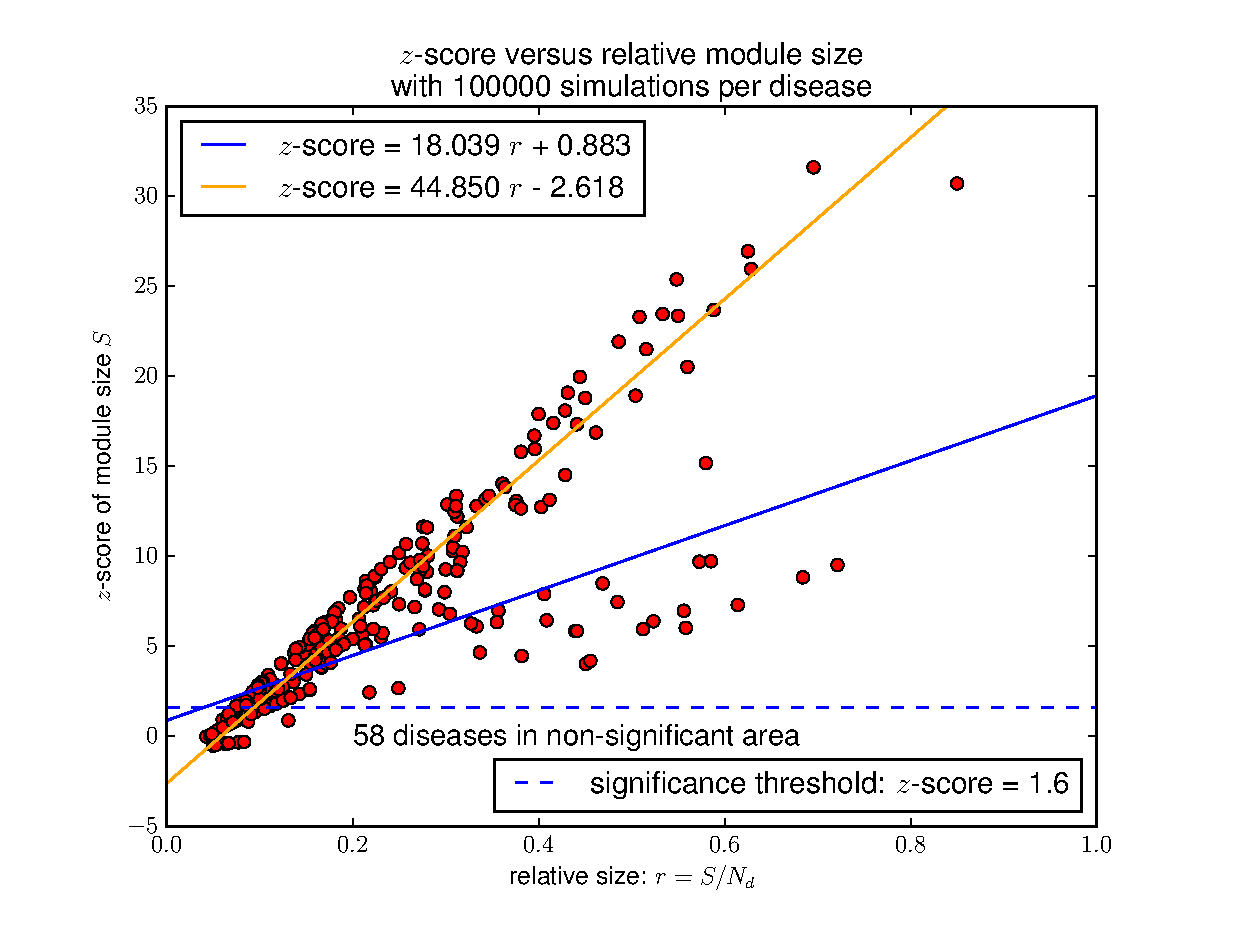
\includegraphics[width=.5\textwidth]{images/S4.b100000.eps}
		\caption{z-score of largest connected component size vs relative module size.\label{fig:zscore}}
	\end{figure}

	\subsection{Separation distribution}
	Original paper's figure 3.K-L plots the separation distribution of the disease pairs according to their
	overlapping score ($C$-score and $J$-score defined respectively as $\abs {A \cap B}/\min(\abs A, \abs B)$ and
	$\abs {A \cap B}/\abs {A \cup B}$ for $A$ and $B$ two diseases). Disease pairs $AB$ having a null $J$-score
	(and thus $C$-score) do not share any gene since $\abs {A \cap B} = 0$. Disease pairs $AB$ having a $C$-score
	equal to 1 are either identical (if their $J$-score equals 1) or one is a strict subset of the other.

	\begin{figure*}[!ht]
		\hspace{-1.8cm}
		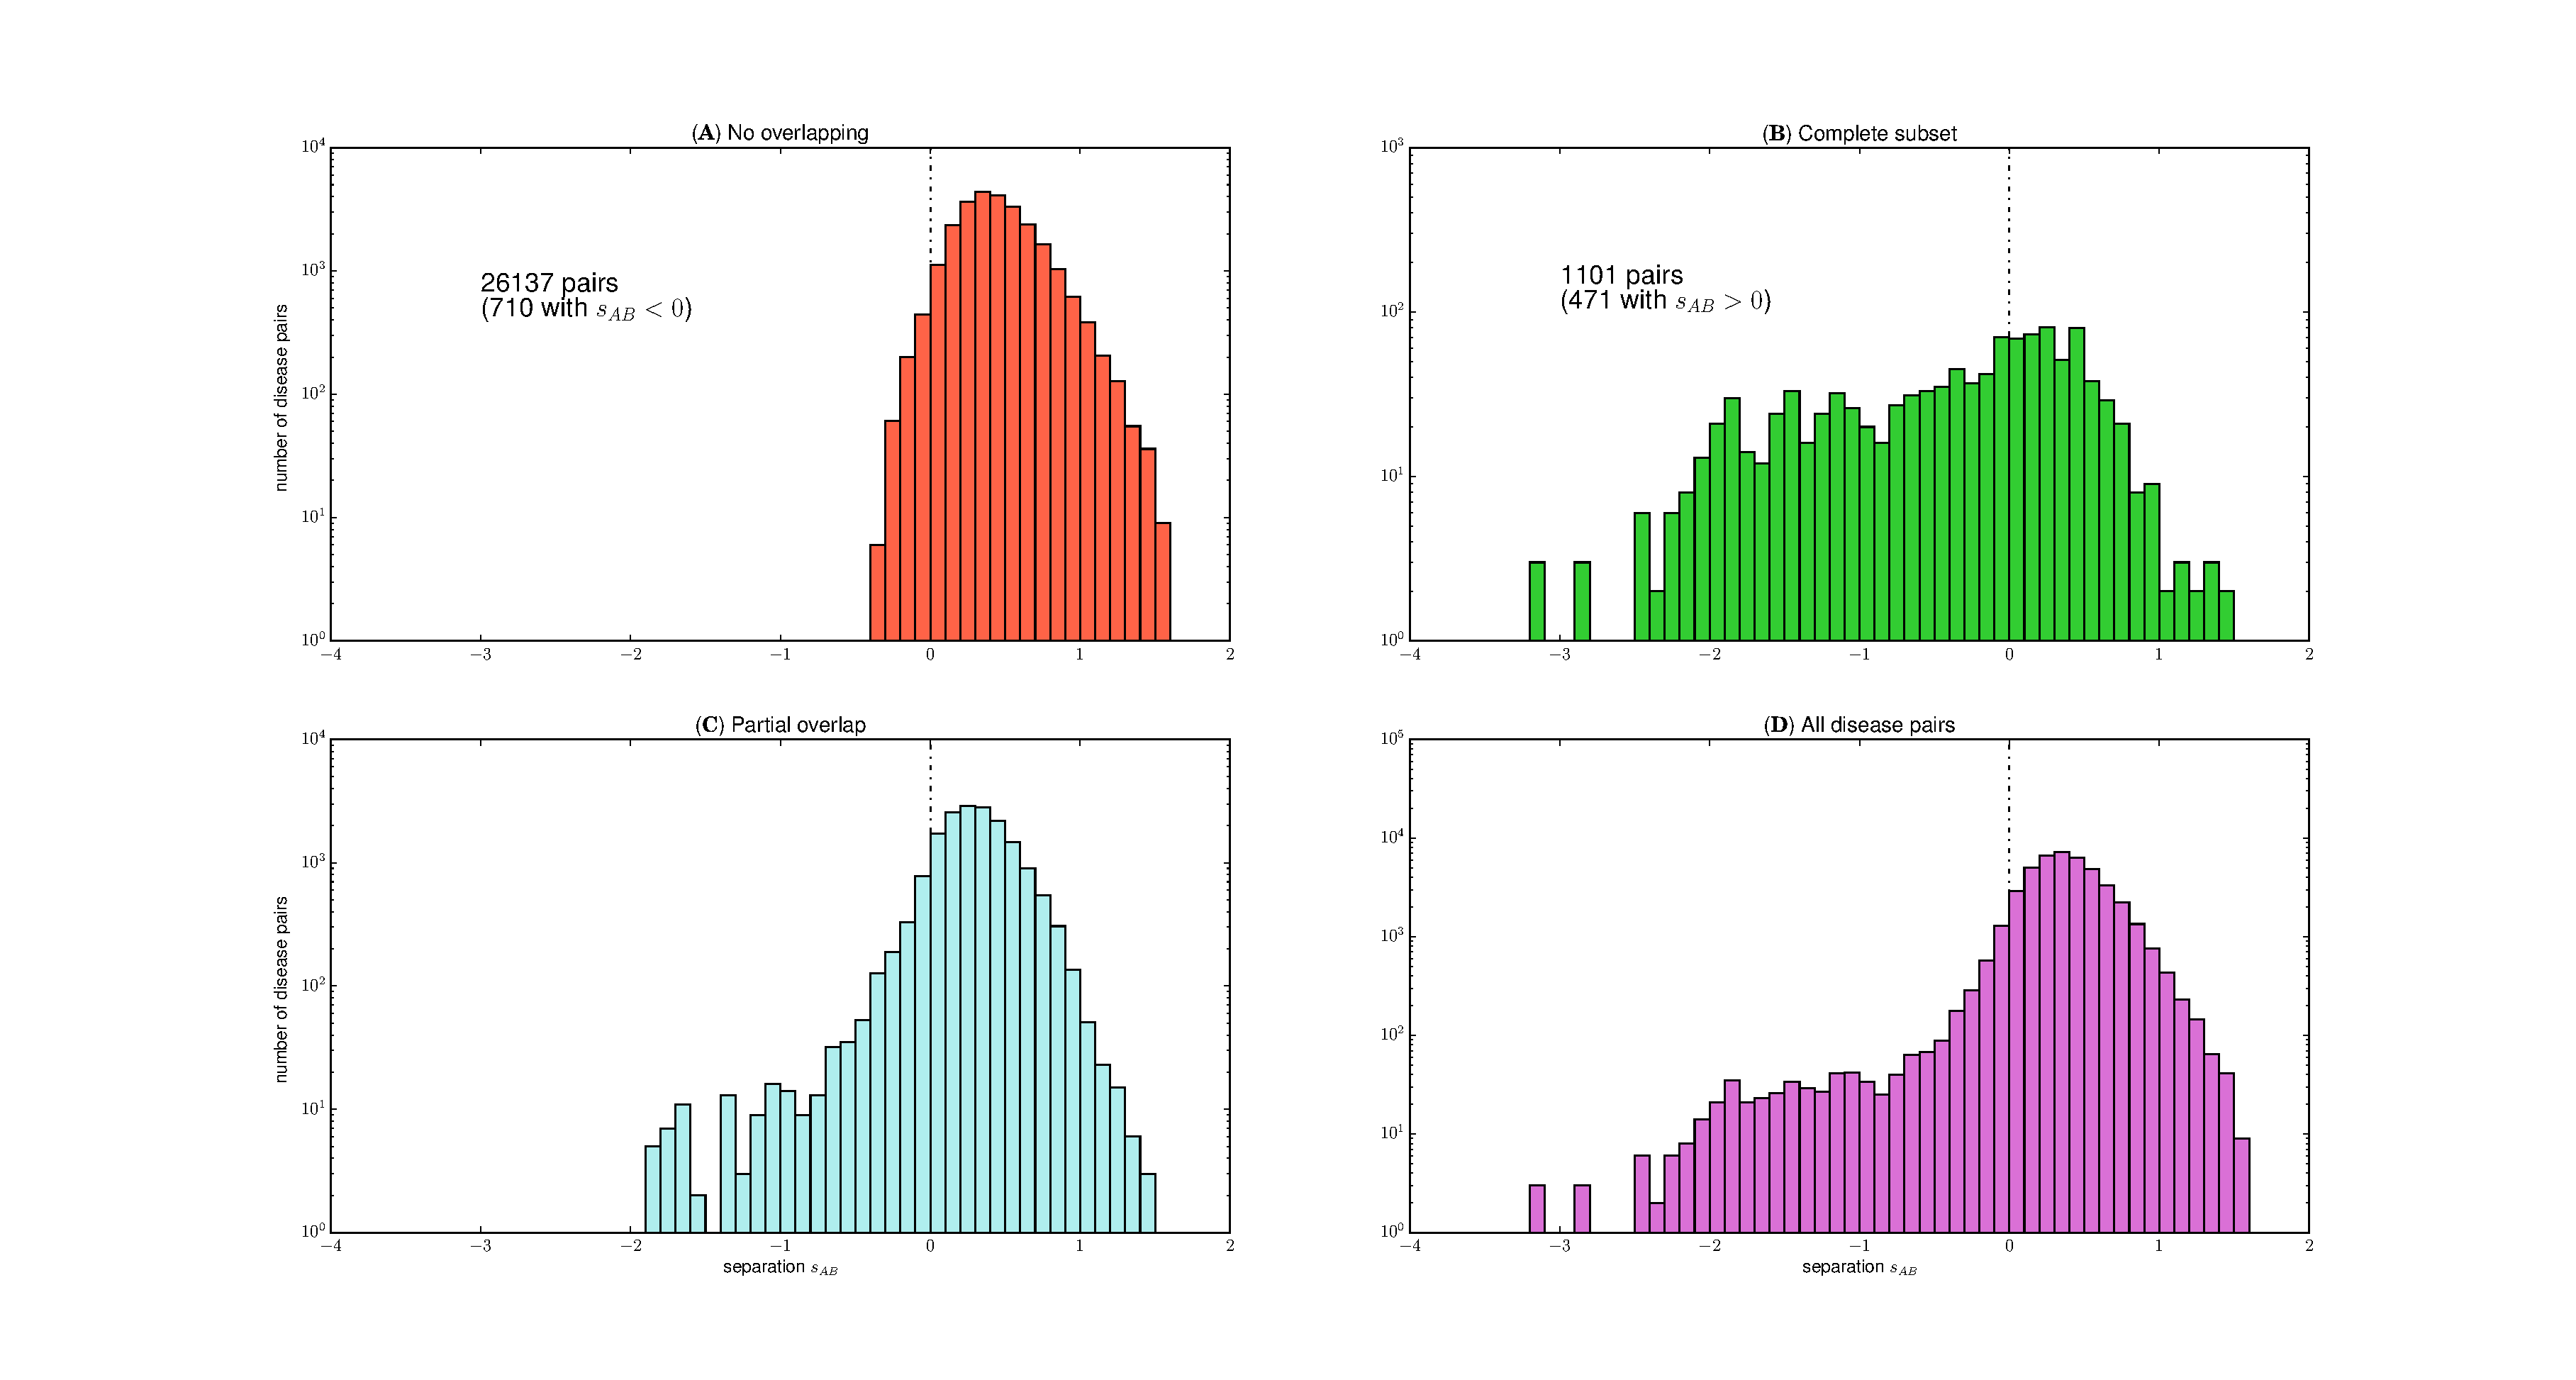
\includegraphics[scale=.35]{images/s_AB_histograms.eps}
		\caption{Disease pairs separation.\label{fig:s_AB histogram}}
	\end{figure*}

	Figure~\ref{fig:s_AB histogram} plots the distribution of $s_{AB}$ separation indicator.
	Distribution shown on ({\bf A}) and ({\bf B}) fit almost exactly the one presented in the article, the only difference
	being that for non-overlapping disease pairs, the amount of pairs having a separation value below 0 is $710$
	versus $717$ in the original paper, being totally non-significant since $7$ pairs represent less than
	$3\%$ of all the non-overlapping pairs set.


\section{Databases update}

	\subsection{Interactome update}
	In order to update the interactome, the tool \textit{inter-tool} presented in~\cite{inter-tools} has
	been used. Latest datasets from BioGRID, IntACT, and the Database of Interacting Proteins (DIP)
	(on July 25th) and of MINT (on July 27th) have been downloaded and merged via inter-tools. This newer
	version merged with the original interactome yield a new graph having 17786 nodes and 370326 edges
	(so a bit more than 1.3 times the initial amount of nodes, and more than 2.6 times the initial amount of edges).

	\subsection{Disease genes update}
	Disease genes considered in this update are the same 299 diseases studied in~\cite{originalPaper}. An update of these
	is yet to be done in further investigations.

	\subsection{Updated results}
	By defining the density of a graph $\Gamma = (V, E)$ as being $d(\Gamma) \coloneqq \abs E/\binom {\abs V}2$,
	we find that the newer interactome is more than 1.5 times denser than the one used in~\cite{originalPaper}.

	\begin{figure}[!h]
		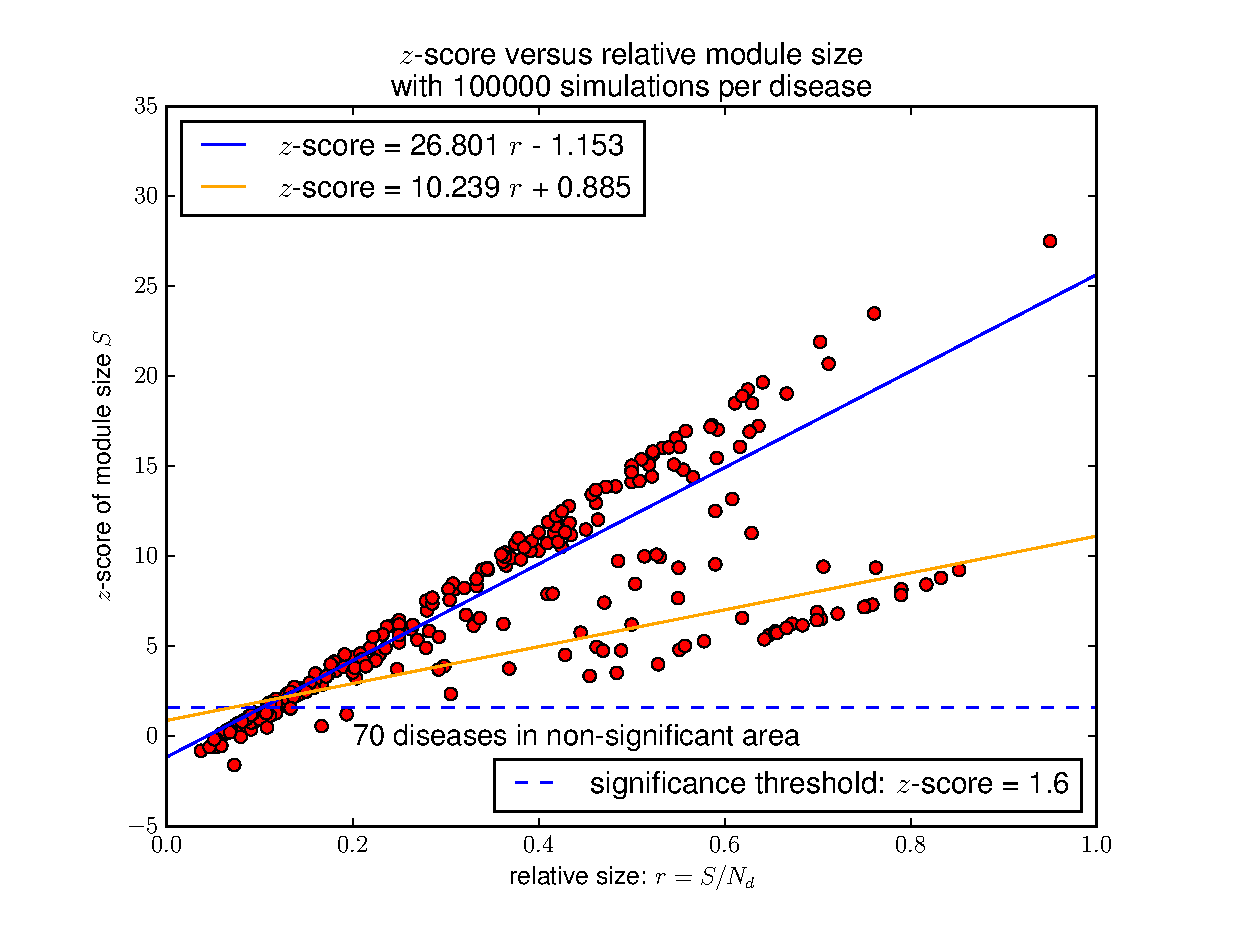
\includegraphics[width=.5\textwidth]{images/new_interactome_S4.b100000.eps}
		\caption{z-score of the largest connected component size vs relative module size of the newer interactome
		\label{fig:new interactome zscore}}
	\end{figure}

	Figure~\ref{fig:new interactome zscore} is the adaptation of Figure~\ref{fig:zscore} for the newer interactome.
	We observe that 12 more diseases have a $z$-score below the threshold of $1.6$, which makes results less significant,
	whereas general relative size has shifted towards right as seen in Figure~\ref{fig:rel sizes comparison}. This
	is explained by the increase in the gene number, leading to a higher coverage of the disease genes.

	\begin{figure}[!h]
		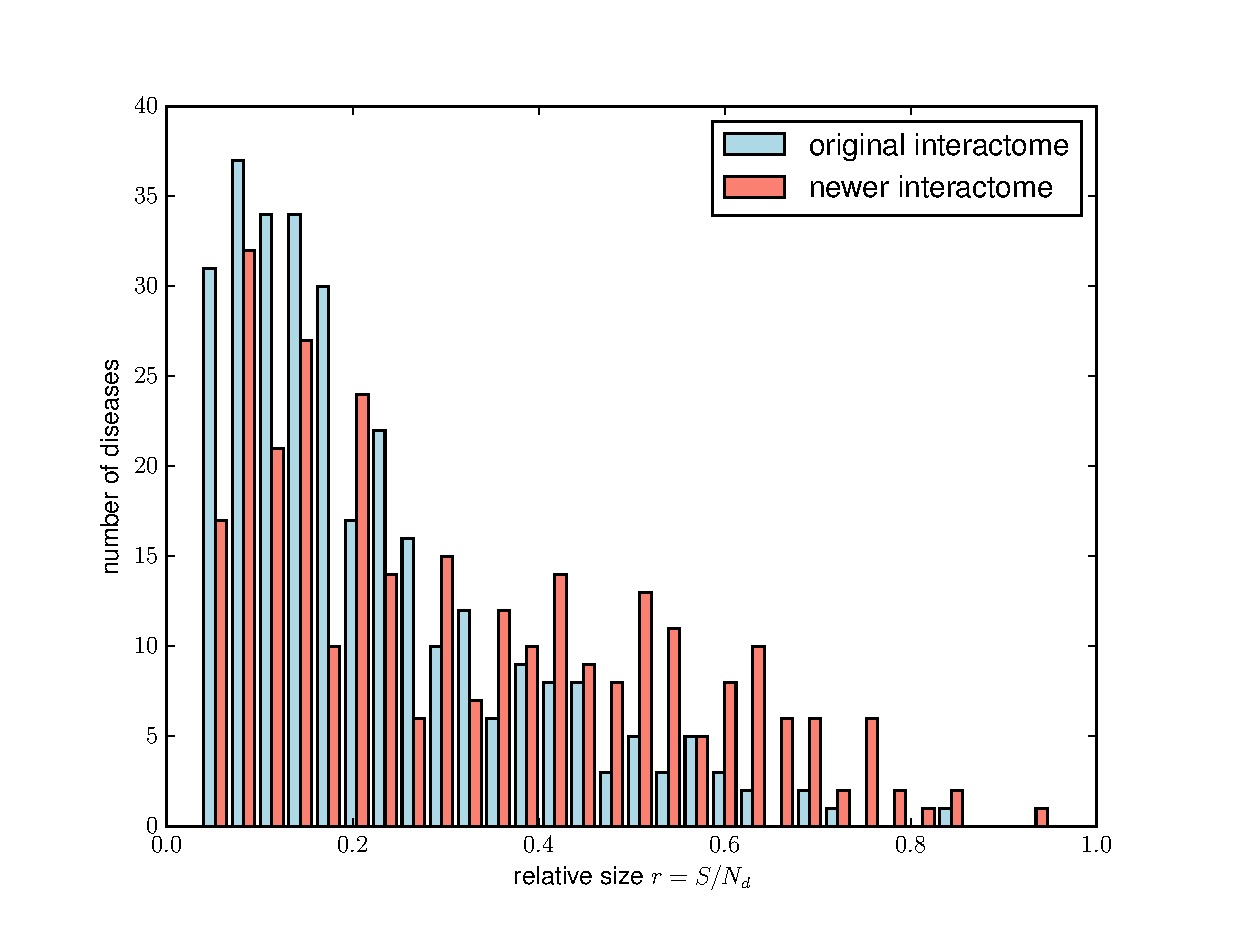
\includegraphics[width=.5\textwidth]{images/rel_sizes_comparison.eps}
		\caption{Comparison of relative size distribution between original and newer interactomes.\label{fig:rel sizes comparison}}
	\end{figure}

	Due to the density increase, the degree distribution has changed as well. Figure~\ref{fig:degree distribution comparison}
	shows the degree distribution of both the original interactome and the new one. The most visible change is that the newer
	interactome contains more connected nodes which implies a mean twice as big.

	\begin{figure}[!h]
		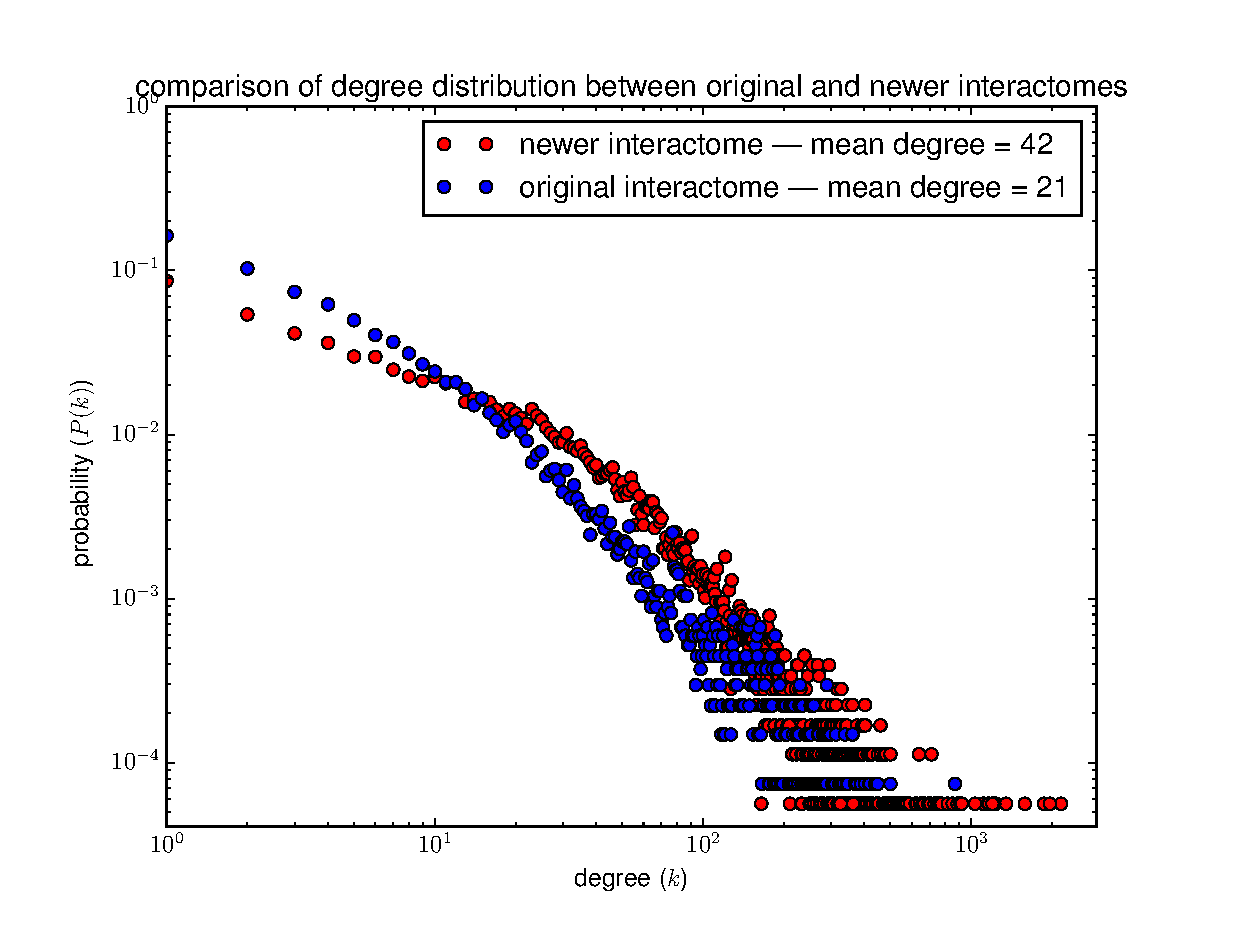
\includegraphics[width=.5\textwidth]{images/degree_distributions_comparison.eps}
		\caption{Degree distribution comparison.\label{fig:degree distribution comparison}}
	\end{figure}

	The 12 diseases which have a decrease of $z$-score below 1.6 is due to the increase of the interactome density implying
	that a subgraph taken at random tends to have a wider LCC at equal size.

\section{Interpretation}

\section{Improvements}

	\subsection{Subgraph largest connected component distribution}
	The $z$-score plotted in Figure~\ref{fig:zscore} requires a null hypothesis, being the random one.
	Those are computed as follows: if $S_D$ is the disease module associated with a given disease $D$,
	then its $z$-score is given by:
	\begin{equation}
		z\text{-score} = \frac {\abs {S_D} - \mu(S^{\text{rand}})}{\sigma(S^{\text{rand}})},
	\end{equation}
	with $\mu(S^{\text{rand}})$ and $\sigma(S^{\text{rand}})$ being respectively the mean and the
	standard deviation of the largest connected component size of a random subgraph of size $\abs D$
	in the interactome.

	These values are obtained by simulations: taking subgraphs at random of given size in the
	interactome. With $10^3$ simulations per subgraph size, Figure~\ref{fig:Srand distribution}
	plots simulated mean and standard deviations of largest connected component size versus
	subgraph size.

	\begin{figure}[!h]\centering
		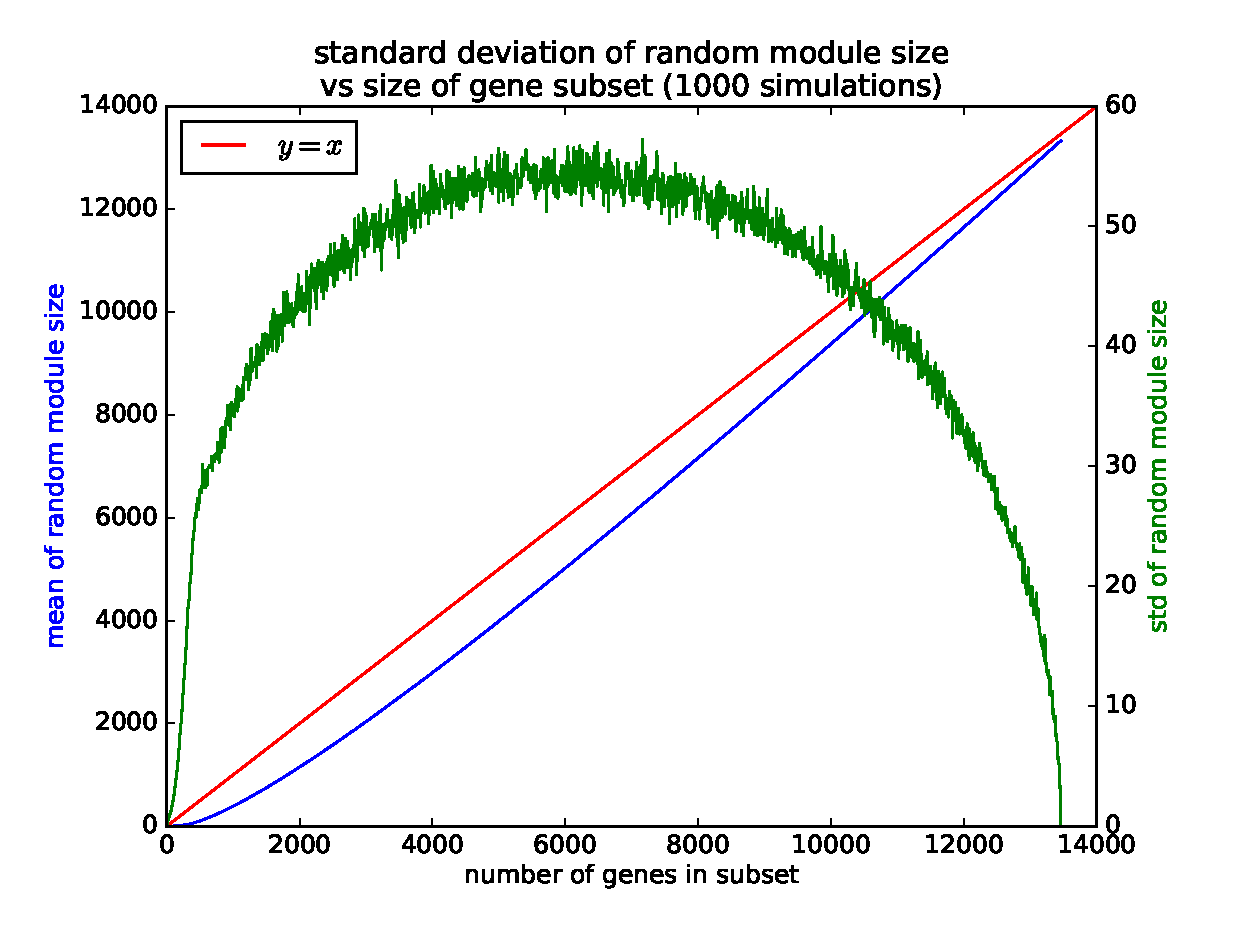
\includegraphics[width=.45\textwidth]{images/Srand_distribution_1000_sims.eps}
		\caption{$S^{\text{rand}}$ mean and standard deviation distribution.\label{fig:Srand distribution}}
	\end{figure}

	% \subsection{Analytically determined probability density}
	% Explain the theoretical method for computing the expected largest connected component size and
	% explain that it is too slow to be used

\section{Conclusion}

\footnotesize
\bibliographystyle{apalike}
\bibliography{report}{}

\end{document}
